\documentclass[12pt, a4paper, hidelinks]{article}

% Packages:
\usepackage{graphicx}                   % For figure includes
\usepackage[T1]{fontenc}                % For mixing up \textsc{} with \textbf{}
\usepackage[utf8]{inputenc}             % For scandinavian input characters(æøå)
\usepackage{amsfonts, amsmath, amssymb} % For common mathsymbols and fonts
\usepackage[danish]{babel}              % For danish titles
\usepackage{hyperref}                   % For making links and refrences
\usepackage{url}                        % Just because {~_^}
\usepackage{array}                      % ...
\usepackage[usenames, dvipsnames, svgnames, table]{xcolor}
\usepackage{tabularx, colortbl}
\usepackage{verbatim} % For entering code snippets.
\usepackage{fancyvrb} % A "fancy" verbatim (for pseudo code).
\usepackage{listings} % For boxed codesnippets, and file includes. (begin)
\usepackage{lipsum}   % For generating dummy text at this demonstration
\usepackage{tikz-qtree,tikz-qtree-compat}
\usepackage{tikz}
\usepackage{enumitem}
\usepackage[simplified]{pgf-umlcd}
\usepackage{float}
\usepackage{feynmp}
\usepackage[shellescape, latex]{gmp}

\usetikzlibrary{trees}
\usetikzlibrary{shapes}

% Basic layout:
\setlength{\textwidth}{165mm}
\setlength{\textheight}{240mm}
\setlength{\parindent}{0mm}
\setlength{\parskip}{\parsep}
\setlength{\headheight}{0mm}
\setlength{\headsep}{0mm}
\setlength{\hoffset}{-2.5mm}
\setlength{\voffset}{0mm}
\setlength{\footskip}{15mm}
\setlength{\oddsidemargin}{0mm}
\setlength{\topmargin}{0mm}
\setlength{\evensidemargin}{0mm}

\newcolumntype{C}[1]{>{\centering\arraybackslash}p{#1}}

% Colors:
\definecolor{KU-red}{RGB}{144, 26, 30}

% Text Coloring:
\newcommand{\green}[1]{\textbf{\color{green}{#1}}}
\newcommand{\blue} [1]{\textbf{\color{blue} {#1}}}
\newcommand{\red}  [1]{\textbf{\color{red}  {#1}}}

% Simple Language Highlighting for F#
\definecolor{bluekeywords}{rgb}{0.13,0.13,1}
\definecolor{greencomments}{rgb}{0,0.5,0}
\definecolor{turqusnumbers}{rgb}{0.17,0.57,0.69}
\definecolor{redstrings}{rgb}{0.5,0,0}
\lstdefinelanguage{FSharp}
                  {morekeywords={let, new, match, with, rec, open,
                      module, namespace, type, of, member, and, for,
                      in, do, begin, end, fun, function, try, mutable,
                      if, then, else},
                    keywordstyle=\color{bluekeywords},
                    sensitive=false,
                    morecomment=[l][\color{greencomments}]{///},
                    morecomment=[l][\color{greencomments}]{//},
                    morecomment=[s][\color{greencomments}]{{(*}{*)}},
                    morestring=[b]",     stringstyle=\color{redstrings}
                  }
% You might want to change these lines at some point
\lstset{
  basicstyle=\ttfamily,
  columns=fullflexible,
  keepspaces=true,
  language=FSharp
}

% ************************* Start Document *****************
\begin{document}

% ************************* Page Header ********************
\begin{minipage}[b]{1.0\linewidth}

\includegraphics[height=30mm]{KULogo}

\vspace*{-16ex}
\begin{center}
    {\Large \bf Programmering og Problemløsning} \vspace*{1ex} \\
    {\large opgave 12} \vspace*{1ex} \\
    {\large Frederik Kallestrup Mastratisi}
\end{center}
\vspace*{-3pt}
{\color{KU-red}\hrule}
\end{minipage}
\vspace{2ex}

% **************** Assignment Starts Here ******************
\tableofcontents \newpage

\section{Overvejelser og valg gjort ved udvikling af programmet}
\setlist[description]{style=nextline}
\begin{description} 

\item[Skabelse af spande]
  I opgave beskrivelsen står der at alle søjler skal have samme bredde, altså at de skal udspænde lige store mængder. Derfor vælger jeg at se det som at jeg ikke kan lade brugeren dele sin sortering op i ethvert antal spande, men i stedet kun de antal som går op i 256, som er størrelse på universet når det kommer til grayscale.

\item[Rendering af histogtammet på skærmen]
Jeg vil gerne have at brugeren selv kan vælge hvor stor firkanten som histogtammet er inde i skal være, dog med en minimum størrelse.

Dette gør dog så jeg ikke kan hard-code akserne ind i programmet. I stedet har jeg skabt en metode hvorved de kan genereres dynamisk. Programmet kan også selv vælge hvilket indkrementering der er bedst at bruge, ud fra nogle valgmuligheder som jeg giver den (disse valgmuligheder kan også let skiftes). Den vælger den valgmulighed som giver den mindste indkrementering, som dog ikke skaber rod skaber rod på akserne.

Det ville ikke kræve meget mere kode, at gøre således at brugeren kunne ændre på størrelsen af histogtammet i real-time!



\end{description}

\section{Bilag}

\begin{figure}[!ht]
  \centering
  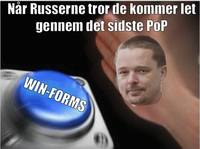
\includegraphics{FriskFraDikuMemes_mini}
  \caption{Miniature af billedet brugt i opgaven}
\end{figure}

\begin{figure}[!ht]
  \centering
  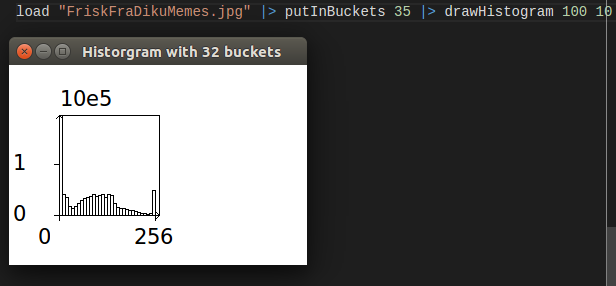
\includegraphics{200x200_32Buckets}
  \caption{Histogram, 200x200, 32 søjler}
\end{figure}

\begin{figure}[!ht]
  \centering
  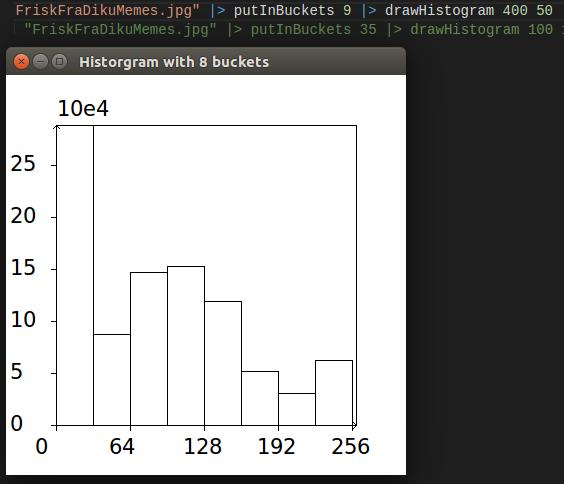
\includegraphics{400x400_8Buckets}
  \caption{Histogram, 400x400, 8 søjler}
\end{figure}

\end{document}